%% here. Need to make the problem description and solution to E.6 and F.6 look like B.6 and C.6

From HW~E.5, the linearized equations of motion are given by
\[
\begin{pmatrix}
m_1 & 0 \\ 0 & \left( \frac{m_2 \ell^2}{3} + m_1 z_e^2 \right)
\end{pmatrix} \begin{pmatrix}\ddot{\tilde{z}} \\ \ddot{\tilde{\theta}} \end{pmatrix}
= \begin{pmatrix} -m_1 g \tilde{\theta} \\ \ell \tilde{F} - m_1 g \tilde{z} \end{pmatrix}.
\]
Inverting the matrix on the left and side gives
\begin{align*}
\begin{pmatrix}\ddot{\tilde{z}} \\ \ddot{\tilde{\theta}} \end{pmatrix}
&= \begin{pmatrix}
	m_1 & 0 \\ 0 & \left( \frac{m_2 \ell^2}{3} + m_1 z_e^2 \right)
	\end{pmatrix}^{-1} \begin{pmatrix} -m_1 g \tilde{\theta} \\ \ell \tilde{F} - m_1 g \tilde{z} \end{pmatrix} \\
&= \begin{pmatrix}
	\frac{1}{m_1} & 0 \\ 0 & \frac{1}{\left( \frac{m_2 \ell^2}{3} + m_1 z_e^2 \right)}
	\end{pmatrix} \begin{pmatrix} -m_1 g \tilde{\theta} \\ \ell \tilde{F} - m_1 g \tilde{z} \end{pmatrix} \\
&= \begin{pmatrix} -g \tilde{\theta} \\ \frac{\ell \tilde{F} - m_1 g \tilde{z}}{\left( \frac{m_2 \ell^2}{3} + m_1 z_e^2 \right)} \end{pmatrix} 
\end{align*}
or in other words, the coupled differential equations
\begin{align*}
\ddot{\tilde{z}} &= -g \tilde{\theta} \\ 
\ddot{\tilde{\theta}} &= -\frac{m_1 g}{\left( \frac{m_2 \ell^2}{3} + m_1 z_e^2 \right)}\tilde{z} + \frac{\ell}{\left( \frac{m_2 \ell^2}{3} + m_1 z_e^2 \right)} \tilde{F}.
\end{align*}
Taking the Laplace transform with initial conditions set to zero and rearranging gives
\begin{align}
s^2 Z(s) &= - g \tilde{\Theta}(s) \label{eq:soln_E6_1}\\
s^2 \tilde{\Theta}(s) &= \frac{\ell}{\frac{m_2 \ell^2}{3} + m_1 z_e^2} \tilde{F}(s) - \frac{m_1 g}{\frac{m_2 \ell^2}{3} + m_1 z_e^2} \tilde{Z}(s).
\label{eq:soln_E6_2}
\end{align}

To simplify the notation in the following discussion, define
\[
A \defeq \frac{m_2 \ell^2}{3} + m_1 z_e^2.
\]
To find the transfer matrix from $\tilde{F}$ to $(\tilde{Z}, \tilde{\Theta})^\top$, write Equation~\eqref{eq:soln_E6_1} and~\eqref{eq:soln_E6_2} in matrix form as
\[
\left(\begin{array}{c|c}
s^2 & -g \\\hline -\frac{m_1g}{A} & s^2 \end{array}\right)
\begin{pmatrix}\tilde{Z}(s) \\ \tilde{\Theta}(s) \end{pmatrix} 
= \begin{pmatrix} 0 \\ \frac{\ell}{A} \end{pmatrix} \tilde{F}(s),
\]
and invert the matrix on the left hand side to obtain
\[
\begin{pmatrix}\tilde{Z}(s) \\ \tilde{\Theta}(s) \end{pmatrix} 
= \begin{pmatrix} 
\frac{-g/A}{s^4-m_1g^2/A} \\ \frac{s^2/A}{s^4-m_1g^2/A}
\end{pmatrix} \tilde{F}(s).
\]

Returning to Equations~\eqref{eq:soln_E6_1} and~\eqref{eq:soln_E6_2} we see that the equations are already in cascade form
\begin{align*}
Z(s) &= -\frac{g}{s^2} \tilde{\Theta}(s) \\
\tilde{\Theta}(s) &= \frac{\left(\frac{\ell}{A}\right)}{s^2} \tilde{F}(s) + D(s)
\end{align*}
where
\[
D(s) = -\frac{\left(\frac{m_1 g}{A}\right)}{s^2} \tilde{Z}(s)
\]
is treated as an unknown disturbance.
The block diagram for the approximate system is shown in Figure~\ref{fig:hw_ballbeam_block_diagram}
\begin{figure}[htbp]
   \centering
   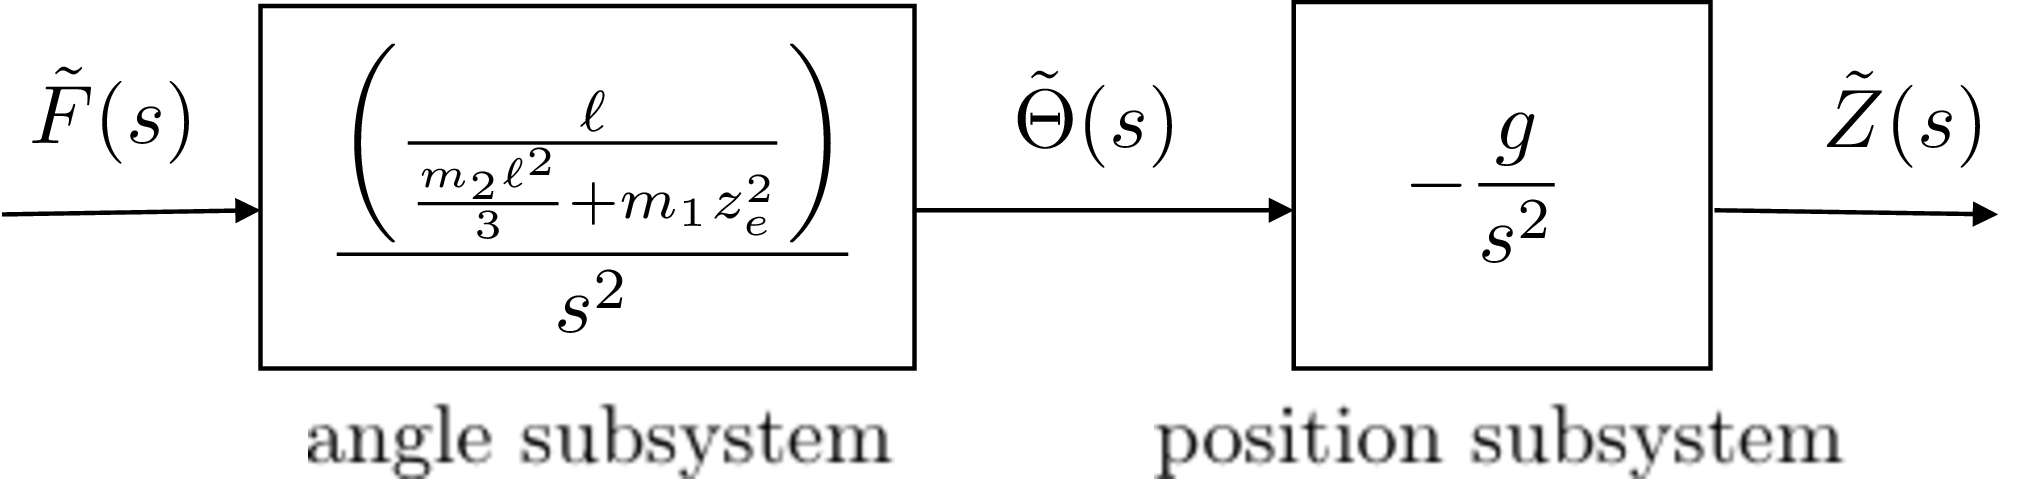
\includegraphics[width=0.8\textwidth]{6_design_studies/figures/hw_ballbeam_block_diagram.pdf}
   \caption{The ball on beam dynamics are approximated by cascade of fast and slow subsystems.  The fast subsystem is the transfer function from the force to the angle, and the slow subsystem is the transfer function from the angle to the position.}
   \label{fig:hw_ballbeam_block_diagram}
\end{figure}

The cascade approximation makes since physically because the force on the beam has an almost immediate effect on the angle of the beam.  
The angle of the beam, then effects the position of the ball.
